\documentclass[]{article}
\usepackage{lmodern}
\usepackage{amssymb,amsmath}
\usepackage{ifxetex,ifluatex}
\usepackage{fixltx2e} % provides \textsubscript
\ifnum 0\ifxetex 1\fi\ifluatex 1\fi=0 % if pdftex
  \usepackage[T1]{fontenc}
  \usepackage[utf8]{inputenc}
\else % if luatex or xelatex
  \ifxetex
    \usepackage{mathspec}
  \else
    \usepackage{fontspec}
  \fi
  \defaultfontfeatures{Ligatures=TeX,Scale=MatchLowercase}
\fi
% use upquote if available, for straight quotes in verbatim environments
\IfFileExists{upquote.sty}{\usepackage{upquote}}{}
% use microtype if available
\IfFileExists{microtype.sty}{%
\usepackage{microtype}
\UseMicrotypeSet[protrusion]{basicmath} % disable protrusion for tt fonts
}{}
\usepackage[margin=1in]{geometry}
\usepackage{hyperref}
\hypersetup{unicode=true,
            pdftitle={Technical Potential of Demand Response},
            pdfauthor={Carsten Dortans (xxx@otago.ac.nz)},
            pdfborder={0 0 0},
            breaklinks=true}
\urlstyle{same}  % don't use monospace font for urls
\usepackage{color}
\usepackage{fancyvrb}
\newcommand{\VerbBar}{|}
\newcommand{\VERB}{\Verb[commandchars=\\\{\}]}
\DefineVerbatimEnvironment{Highlighting}{Verbatim}{commandchars=\\\{\}}
% Add ',fontsize=\small' for more characters per line
\usepackage{framed}
\definecolor{shadecolor}{RGB}{248,248,248}
\newenvironment{Shaded}{\begin{snugshade}}{\end{snugshade}}
\newcommand{\KeywordTok}[1]{\textcolor[rgb]{0.13,0.29,0.53}{\textbf{#1}}}
\newcommand{\DataTypeTok}[1]{\textcolor[rgb]{0.13,0.29,0.53}{#1}}
\newcommand{\DecValTok}[1]{\textcolor[rgb]{0.00,0.00,0.81}{#1}}
\newcommand{\BaseNTok}[1]{\textcolor[rgb]{0.00,0.00,0.81}{#1}}
\newcommand{\FloatTok}[1]{\textcolor[rgb]{0.00,0.00,0.81}{#1}}
\newcommand{\ConstantTok}[1]{\textcolor[rgb]{0.00,0.00,0.00}{#1}}
\newcommand{\CharTok}[1]{\textcolor[rgb]{0.31,0.60,0.02}{#1}}
\newcommand{\SpecialCharTok}[1]{\textcolor[rgb]{0.00,0.00,0.00}{#1}}
\newcommand{\StringTok}[1]{\textcolor[rgb]{0.31,0.60,0.02}{#1}}
\newcommand{\VerbatimStringTok}[1]{\textcolor[rgb]{0.31,0.60,0.02}{#1}}
\newcommand{\SpecialStringTok}[1]{\textcolor[rgb]{0.31,0.60,0.02}{#1}}
\newcommand{\ImportTok}[1]{#1}
\newcommand{\CommentTok}[1]{\textcolor[rgb]{0.56,0.35,0.01}{\textit{#1}}}
\newcommand{\DocumentationTok}[1]{\textcolor[rgb]{0.56,0.35,0.01}{\textbf{\textit{#1}}}}
\newcommand{\AnnotationTok}[1]{\textcolor[rgb]{0.56,0.35,0.01}{\textbf{\textit{#1}}}}
\newcommand{\CommentVarTok}[1]{\textcolor[rgb]{0.56,0.35,0.01}{\textbf{\textit{#1}}}}
\newcommand{\OtherTok}[1]{\textcolor[rgb]{0.56,0.35,0.01}{#1}}
\newcommand{\FunctionTok}[1]{\textcolor[rgb]{0.00,0.00,0.00}{#1}}
\newcommand{\VariableTok}[1]{\textcolor[rgb]{0.00,0.00,0.00}{#1}}
\newcommand{\ControlFlowTok}[1]{\textcolor[rgb]{0.13,0.29,0.53}{\textbf{#1}}}
\newcommand{\OperatorTok}[1]{\textcolor[rgb]{0.81,0.36,0.00}{\textbf{#1}}}
\newcommand{\BuiltInTok}[1]{#1}
\newcommand{\ExtensionTok}[1]{#1}
\newcommand{\PreprocessorTok}[1]{\textcolor[rgb]{0.56,0.35,0.01}{\textit{#1}}}
\newcommand{\AttributeTok}[1]{\textcolor[rgb]{0.77,0.63,0.00}{#1}}
\newcommand{\RegionMarkerTok}[1]{#1}
\newcommand{\InformationTok}[1]{\textcolor[rgb]{0.56,0.35,0.01}{\textbf{\textit{#1}}}}
\newcommand{\WarningTok}[1]{\textcolor[rgb]{0.56,0.35,0.01}{\textbf{\textit{#1}}}}
\newcommand{\AlertTok}[1]{\textcolor[rgb]{0.94,0.16,0.16}{#1}}
\newcommand{\ErrorTok}[1]{\textcolor[rgb]{0.64,0.00,0.00}{\textbf{#1}}}
\newcommand{\NormalTok}[1]{#1}
\usepackage{longtable,booktabs}
\usepackage{graphicx,grffile}
\makeatletter
\def\maxwidth{\ifdim\Gin@nat@width>\linewidth\linewidth\else\Gin@nat@width\fi}
\def\maxheight{\ifdim\Gin@nat@height>\textheight\textheight\else\Gin@nat@height\fi}
\makeatother
% Scale images if necessary, so that they will not overflow the page
% margins by default, and it is still possible to overwrite the defaults
% using explicit options in \includegraphics[width, height, ...]{}
\setkeys{Gin}{width=\maxwidth,height=\maxheight,keepaspectratio}
\IfFileExists{parskip.sty}{%
\usepackage{parskip}
}{% else
\setlength{\parindent}{0pt}
\setlength{\parskip}{6pt plus 2pt minus 1pt}
}
\setlength{\emergencystretch}{3em}  % prevent overfull lines
\providecommand{\tightlist}{%
  \setlength{\itemsep}{0pt}\setlength{\parskip}{0pt}}
\setcounter{secnumdepth}{5}
% Redefines (sub)paragraphs to behave more like sections
\ifx\paragraph\undefined\else
\let\oldparagraph\paragraph
\renewcommand{\paragraph}[1]{\oldparagraph{#1}\mbox{}}
\fi
\ifx\subparagraph\undefined\else
\let\oldsubparagraph\subparagraph
\renewcommand{\subparagraph}[1]{\oldsubparagraph{#1}\mbox{}}
\fi

%%% Use protect on footnotes to avoid problems with footnotes in titles
\let\rmarkdownfootnote\footnote%
\def\footnote{\protect\rmarkdownfootnote}

%%% Change title format to be more compact
\usepackage{titling}

% Create subtitle command for use in maketitle
\newcommand{\subtitle}[1]{
  \posttitle{
    \begin{center}\large#1\end{center}
    }
}

\setlength{\droptitle}{-2em}
  \title{Technical Potential of Demand Response}
  \pretitle{\vspace{\droptitle}\centering\huge}
  \posttitle{\par}
\subtitle{Heat Pump Analysis}
  \author{Carsten Dortans
(\href{mailto:xxx@otago.ac.nz}{\nolinkurl{xxx@otago.ac.nz}})}
  \preauthor{\centering\large\emph}
  \postauthor{\par}
  \predate{\centering\large\emph}
  \postdate{\par}
  \date{Last run at: 2018-06-28 10:34:21}


\begin{document}
\maketitle

{
\setcounter{tocdepth}{2}
\tableofcontents
}
\newpage

\section{Citation}\label{citation}

If you wish to use any of the material from this report please cite as:

\begin{itemize}
\tightlist
\item
  Dortans, C. (2018) Technical Potential of Demand Response: Heat Pump
  Analysis, \href{http://www.otago.ac.nz/centre-sustainability/}{Centre
  for Sustainability}, University of Otago: Dunedin.
\end{itemize}

This work is (c) 2018 the University of Southampton.

\newpage

\section{About}\label{about}

\subsection{Circulation}\label{circulation}

Report circulation:

\begin{itemize}
\tightlist
\item
  Restricted to:
  \href{https://www.otago.ac.nz/centre-sustainability/research/energy/otago050285.html}{NZ
  GREEN Grid} project partners and contractors.
\end{itemize}

\subsection{Purpose}\label{purpose}

This report is intended to:

\begin{itemize}
\tightlist
\item
  load and test GREEN Grid heat pump and hot water profiles.
\end{itemize}

\subsection{Requirements:}\label{requirements}

\begin{itemize}
\tightlist
\item
  test dataset stored at
  /Users/carsten.dortans/Dropbox/Carsten\_MA/ggData/profiles/
\end{itemize}

\subsection{History}\label{history}

Generally tracked via our git.soton
\href{https://git.soton.ac.uk/ba1e12/nzGREENGrid}{repo}:

\begin{itemize}
\tightlist
\item
  \href{https://git.soton.ac.uk/ba1e12/nzGREENGrid/commits/master}{history}
\item
  \href{https://git.soton.ac.uk/ba1e12/nzGREENGrid/issues}{issues}
\end{itemize}

Specific history of this code:

\begin{itemize}
\tightlist
\item
  \url{https://git.soton.ac.uk/ba1e12/nzGREENGrid/tree/master/analysis/demandResponse}
\end{itemize}

\subsection{Support}\label{support}

This work was supported by:

\begin{itemize}
\tightlist
\item
  The \href{https://www.otago.ac.nz/}{University of Otago};
\item
  The \href{https://www.southampton.ac.uk/}{University of Southampton};
\item
  The New Zealand \href{http://www.mbie.govt.nz/}{Ministry of Business,
  Innovation and Employment (MBIE)} through the
  \href{https://www.otago.ac.nz/centre-sustainability/research/energy/otago050285.html}{NZ
  GREEN Grid} project;
\item
  \href{http://www.energy.soton.ac.uk/tag/spatialec/}{SPATIALEC} - a
  \href{http://ec.europa.eu/research/mariecurieactions/about-msca/actions/if/index_en.htm}{Marie
  Skłodowska-Curie Global Fellowship} based at the University of Otago's
  \href{http://www.otago.ac.nz/centre-sustainability/staff/otago673896.html}{Centre
  for Sustainability} (2017-2019) \& the University of Southampton's
  Sustainable Energy Research Group (2019-202).
\end{itemize}

We do not `support' the code but if you have a problem check the
\href{https://git.soton.ac.uk/ba1e12/nzGREENGrid/issues}{issues} on our
\href{https://git.soton.ac.uk/ba1e12/nzGREENGrid}{repo} and if it
doesn't already exist, open one. We might be able to fix it :-)

\section{Load data files}\label{load-data-files}

\subsection{Heat pump profiles}\label{heat-pump-profiles}

This file is the pre-aggregated data for all heat pump circuits in the
GREEN Grid data for April 2015 - March 2016 (check!)

\begin{Shaded}
\begin{Highlighting}[]
\NormalTok{ggParams}\OperatorTok{$}\NormalTok{profilesFile <-}\StringTok{ }\KeywordTok{paste0}\NormalTok{(ggParams}\OperatorTok{$}\NormalTok{dataLoc, }\StringTok{"Heat Pump_2015-04-01_2016-03-31_overallSeasonalProfiles.csv.gz"}\NormalTok{)}
\end{Highlighting}
\end{Shaded}

In this section we load and describe the data files from
/Users/carsten.dortans/Dropbox/Carsten\_MA/ggData/profiles/Heat
Pump\_2015-04-01\_2016-03-31\_overallSeasonalProfiles.csv.gz.

\begin{Shaded}
\begin{Highlighting}[]
\KeywordTok{print}\NormalTok{(}\KeywordTok{paste0}\NormalTok{(}\StringTok{"Trying to load: "}\NormalTok{, ggParams}\OperatorTok{$}\NormalTok{profilesFile))}
\end{Highlighting}
\end{Shaded}

\begin{verbatim}
## [1] "Trying to load: /Users/carsten.dortans/Dropbox/Carsten_MA/ggData/profiles/Heat Pump_2015-04-01_2016-03-31_overallSeasonalProfiles.csv.gz"
\end{verbatim}

\begin{Shaded}
\begin{Highlighting}[]
\NormalTok{heatPumpProfileDT <-}\StringTok{ }\NormalTok{data.table}\OperatorTok{::}\KeywordTok{as.data.table}\NormalTok{(readr}\OperatorTok{::}\KeywordTok{read_csv}\NormalTok{(ggParams}\OperatorTok{$}\NormalTok{profilesFile))}
\end{Highlighting}
\end{Shaded}

\begin{verbatim}
## Parsed with column specification:
## cols(
##   obsHourMin = col_time(format = ""),
##   season = col_character(),
##   meanW = col_double(),
##   medianW = col_double(),
##   nObs = col_integer(),
##   sdW = col_double()
## )
\end{verbatim}

Describe using skim:

\begin{Shaded}
\begin{Highlighting}[]
\NormalTok{skimr}\OperatorTok{::}\KeywordTok{skim}\NormalTok{(heatPumpProfileDT)}
\end{Highlighting}
\end{Shaded}

\begin{verbatim}
## Skim summary statistics
##  n obs: 5760 
##  n variables: 6 
## 
## -- Variable type:character -----------------------------------------------------------------------------------------------------------------
##  variable missing complete    n min max empty n_unique
##    season       0     5760 5760   6   6     0        4
## 
## -- Variable type:difftime ------------------------------------------------------------------------------------------------------------------
##    variable missing complete    n    min        max     median n_unique
##  obsHourMin       0     5760 5760 0 secs 86340 secs 43170 secs     1440
## 
## -- Variable type:integer -------------------------------------------------------------------------------------------------------------------
##  variable missing complete    n    mean     sd   p0    p25    p50     p75
##      nObs       0     5760 5760 2474.38 193.08 2150 2402.5 2517.5 2599.25
##  p100     hist
##  2688 ▅▁▁▁▁▇▁▅
## 
## -- Variable type:numeric -------------------------------------------------------------------------------------------------------------------
##  variable missing complete    n   mean     sd     p0    p25    p50    p75
##     meanW       0     5760 5760 143.52 116.99  34.99  71.88 104.76 174.71
##   medianW       0     5760 5760  17.09  67.67   0      0      0      0   
##       sdW       0     5760 5760 329.77 146.05 101.04 234.33 298.61 407.13
##    p100     hist
##  613.89 ▇▃▂▁▁▁▁▁
##  392.55 ▇▁▁▁▁▁▁▁
##  879.07 ▆▇▆▅▂▂▁▁
\end{verbatim}

Draw a plot of GreenGrid heat pump profiles.

\begin{Shaded}
\begin{Highlighting}[]
\NormalTok{myPlot <-}\StringTok{ }\NormalTok{ggplot2}\OperatorTok{::}\KeywordTok{ggplot}\NormalTok{(heatPumpProfileDT, }\KeywordTok{aes}\NormalTok{(}\DataTypeTok{x =}\NormalTok{ obsHourMin, }\DataTypeTok{colour =}\NormalTok{ season)) }\OperatorTok{+}
\StringTok{  }\KeywordTok{geom_point}\NormalTok{(}\KeywordTok{aes}\NormalTok{(}\DataTypeTok{y =}\NormalTok{ meanW)) }\OperatorTok{+}
\StringTok{  }\KeywordTok{facet_grid}\NormalTok{(season }\OperatorTok{~}\StringTok{ }\NormalTok{.)}

\NormalTok{myPlot}
\end{Highlighting}
\end{Shaded}

\begin{figure}
\centering
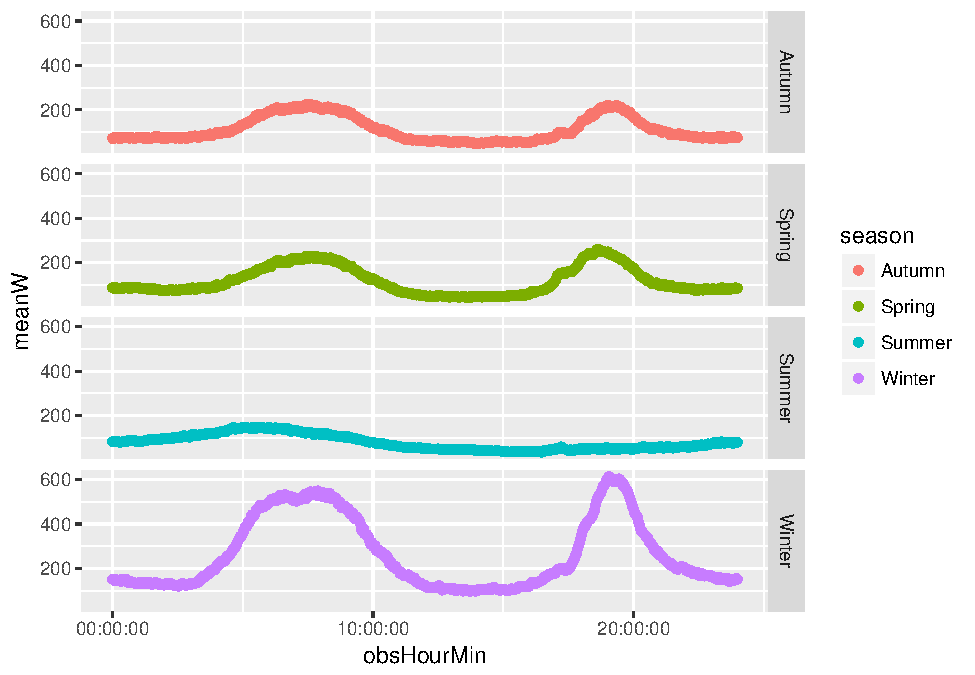
\includegraphics{heatPumpProfileAnalysis_files/figure-latex/profilePlot-1.pdf}
\caption{\label{fig:profilePlot}Heat pump profiles}
\end{figure}

\section{Scaling method 1}\label{scaling-method-1}

Now draw a plot of what woud happen if we scaled this up to all NZ
households?

Figure \ref{fig:scaledUpPlots}

\begin{Shaded}
\begin{Highlighting}[]
\NormalTok{nzHH <-}\StringTok{ }\DecValTok{1549890}

\NormalTok{heatPumpProfileDT <-}\StringTok{ }\NormalTok{heatPumpProfileDT[, scaledMWmethod1 }\OperatorTok{:}\ErrorTok{=}\StringTok{ }\NormalTok{(meanW }\OperatorTok{*}\StringTok{ }\NormalTok{nzHH)}\OperatorTok{/}\DecValTok{10}\OperatorTok{^}\DecValTok{6}\NormalTok{]}

\NormalTok{myPlot <-}\StringTok{ }\NormalTok{ggplot2}\OperatorTok{::}\KeywordTok{ggplot}\NormalTok{(heatPumpProfileDT, }\KeywordTok{aes}\NormalTok{(}\DataTypeTok{x =}\NormalTok{ obsHourMin, }\DataTypeTok{colour =}\NormalTok{ season)) }\OperatorTok{+}
\StringTok{  }\KeywordTok{geom_point}\NormalTok{(}\KeywordTok{aes}\NormalTok{(}\DataTypeTok{y =}\NormalTok{ scaledMWmethod1)) }\OperatorTok{+}
\StringTok{  }\KeywordTok{facet_grid}\NormalTok{(season }\OperatorTok{~}\StringTok{ }\NormalTok{.)}

\NormalTok{myPlot}
\end{Highlighting}
\end{Shaded}

\begin{figure}
\centering
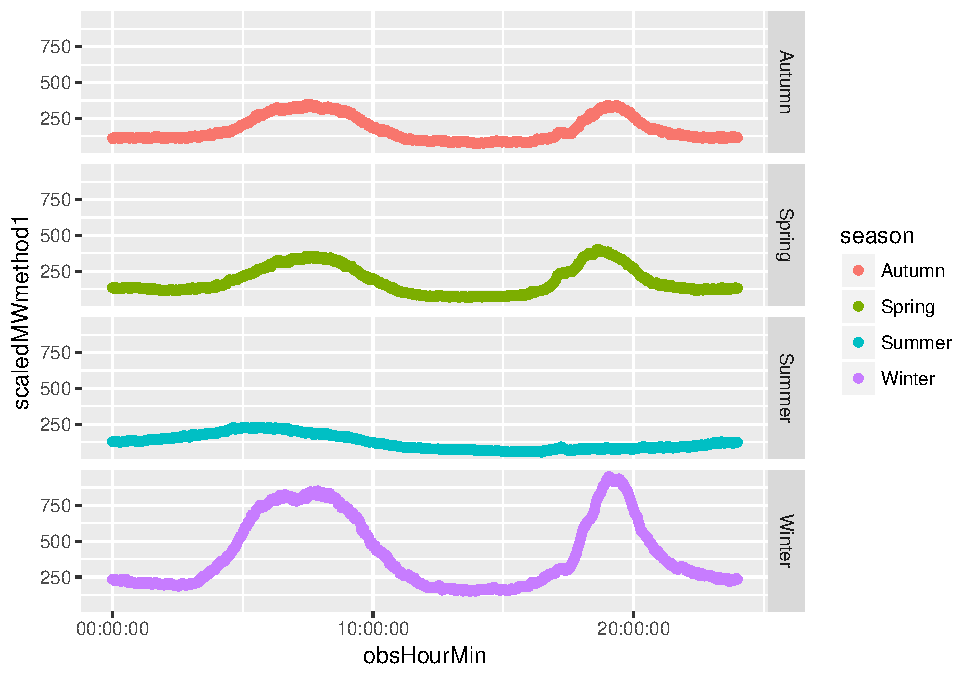
\includegraphics{heatPumpProfileAnalysis_files/figure-latex/scaledUpPlots-1.pdf}
\caption{\label{fig:scaledUpPlots}Mean Load Heat Pumps by Season}
\end{figure}

\section{Scaling method 2}\label{scaling-method-2}

Alternative calculation method: Assuming EECA data is correct for heat
pump value, 1) generating the percentage of total load (peroftotal)
while telling data.table to create a new column with the calculation of
the percentage. We then multiplied EECA's total GWh with the percentage

\begin{Shaded}
\begin{Highlighting}[]
\NormalTok{totalGWH<-}\DecValTok{708}

\NormalTok{summeanW<-heatPumpProfileDT[,}\KeywordTok{sum}\NormalTok{(meanW)]}



\NormalTok{heatPumpProfileDT <-}\StringTok{ }\NormalTok{heatPumpProfileDT[, EECApmMethod2 }\OperatorTok{:}\ErrorTok{=}\StringTok{ }\NormalTok{(meanW }\OperatorTok{/}\StringTok{ }\NormalTok{summeanW) }\OperatorTok{*}\StringTok{ }\NormalTok{totalGWH] }

\NormalTok{myPlot <-}\StringTok{ }\NormalTok{ggplot2}\OperatorTok{::}\KeywordTok{ggplot}\NormalTok{(heatPumpProfileDT, }\KeywordTok{aes}\NormalTok{(}\DataTypeTok{x =}\NormalTok{ obsHourMin, }\DataTypeTok{colour =}\NormalTok{ season)) }\OperatorTok{+}
\StringTok{  }\KeywordTok{geom_point}\NormalTok{(}\KeywordTok{aes}\NormalTok{(}\DataTypeTok{y =}\NormalTok{ EECApmMethod2)) }\OperatorTok{+}
\StringTok{  }\KeywordTok{facet_grid}\NormalTok{(season }\OperatorTok{~}\StringTok{ }\NormalTok{.) }\OperatorTok{+}
\StringTok{  }\KeywordTok{labs}\NormalTok{(}\DataTypeTok{x=}\StringTok{'Time of Day'}\NormalTok{, }\DataTypeTok{y=}\StringTok{'GWh'}\NormalTok{)}

\NormalTok{myPlot}
\end{Highlighting}
\end{Shaded}

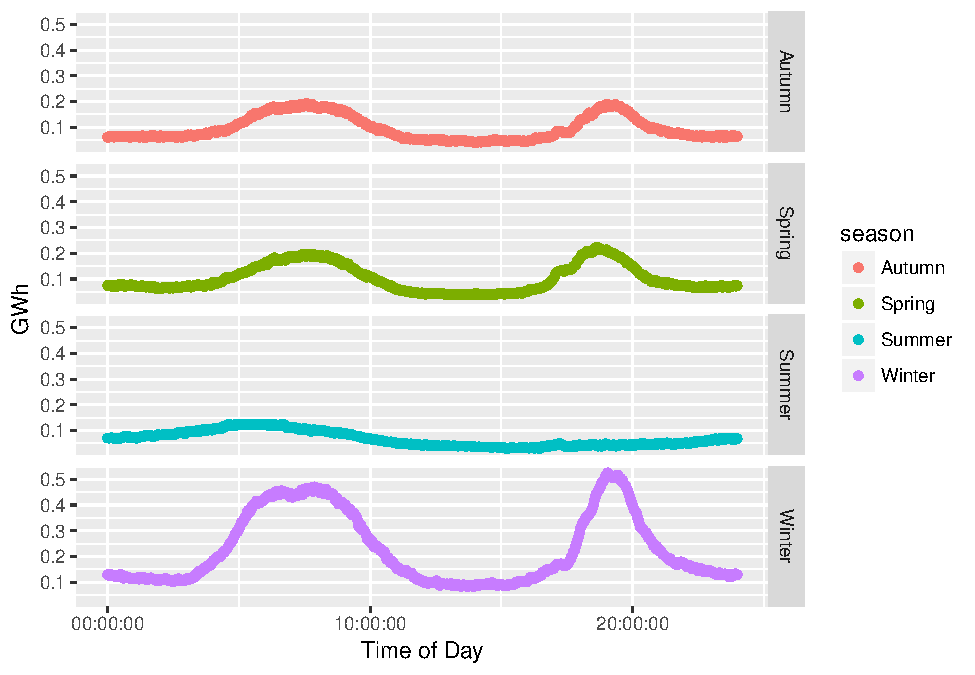
\includegraphics{heatPumpProfileAnalysis_files/figure-latex/new calc-1.pdf}

\section{Aggregation to half-hours}\label{aggregation-to-half-hours}

So far we have used data at the 1 minute level. This makes for
difficulties in comparison with standared electricity sector half-hourly
tariff periods etc. This section takes each scaling method, aggregates
to half-hours as appropriate and re-plots.

To do that we need to set a half-hour value from the observed time. We
do this using truncate so that:

\begin{itemize}
\tightlist
\item
  13:18:00 -\textgreater{} 13:00:00
\item
  13:40:00 -\textgreater{} 13:30 etc
\end{itemize}

\begin{quote}
NB: This means any plots will be using the 1/2 hour value at the
\emph{start} of the period!
\end{quote}

\begin{Shaded}
\begin{Highlighting}[]
\CommentTok{# create a 'half hour' variable for aggregation}
\NormalTok{heatPumpProfileDT <-}\StringTok{ }\NormalTok{heatPumpProfileDT[, obsHalfHour }\OperatorTok{:}\ErrorTok{=}\StringTok{ }\NormalTok{hms}\OperatorTok{::}\KeywordTok{trunc_hms}\NormalTok{(obsHourMin, }\DecValTok{1800}\NormalTok{)] }\CommentTok{# <- this truncates the time to the previous half hour (hms works in seconds so 30 mins * 60 secs = 1800 secs). e.g. 13:18:00 -> 13:00:00 but 13:40:00 -> 13:30 etc}

\CommentTok{# This means any plots will be using the 1/2 hour value at the  -> start <-  of the period!}

\CommentTok{# check}
\KeywordTok{head}\NormalTok{(heatPumpProfileDT)}
\end{Highlighting}
\end{Shaded}

\begin{verbatim}
##    obsHourMin season     meanW medianW nObs      sdW scaledMWmethod1
## 1:   00:00:00 Autumn  72.43808       0 2543 253.7921        112.2711
## 2:   00:00:00 Spring  87.36049       0 2512 289.1072        135.3991
## 3:   00:00:00 Summer  82.63281       0 2160 258.2699        128.0718
## 4:   00:00:00 Winter 150.92446       0 2685 383.6956        233.9163
## 5:   00:01:00 Autumn  70.26538       0 2544 238.4719        108.9036
## 6:   00:01:00 Spring  86.17364       0 2511 286.9992        133.5597
##    EECApmMethod2 obsHalfHour
## 1:    0.06203848    00:00:00
## 2:    0.07481856    00:00:00
## 3:    0.07076961    00:00:00
## 4:    0.12925695    00:00:00
## 5:    0.06017771    00:00:00
## 6:    0.07380210    00:00:00
\end{verbatim}

\subsection{Method 1}\label{method-1}

\begin{Shaded}
\begin{Highlighting}[]
\CommentTok{# aggregate the scaled MW to half hours}
\CommentTok{# as it is MW we need to take the mean - taking the sum would not be meaningfull}
\NormalTok{method1AggDT <-}\StringTok{ }\NormalTok{heatPumpProfileDT[, .(}\DataTypeTok{meanMW =} \KeywordTok{mean}\NormalTok{(scaledMWmethod1)), }
\NormalTok{                                  keyby =}\StringTok{ }\NormalTok{.(season, obsHalfHour)] }\CommentTok{# <- takes the mean for each category of half hour & season}

\NormalTok{myPlot <-}\StringTok{ }\NormalTok{ggplot2}\OperatorTok{::}\KeywordTok{ggplot}\NormalTok{(method1AggDT, }\KeywordTok{aes}\NormalTok{(}\DataTypeTok{x =}\NormalTok{ obsHalfHour, }\DataTypeTok{colour =}\NormalTok{ season)) }\OperatorTok{+}
\StringTok{  }\KeywordTok{geom_point}\NormalTok{(}\KeywordTok{aes}\NormalTok{(}\DataTypeTok{y =}\NormalTok{ meanMW)) }\OperatorTok{+}
\StringTok{  }\KeywordTok{facet_grid}\NormalTok{(season }\OperatorTok{~}\StringTok{ }\NormalTok{.) }\OperatorTok{+}
\StringTok{  }\KeywordTok{labs}\NormalTok{(}\DataTypeTok{x=}\StringTok{'Time of Day'}\NormalTok{, }\DataTypeTok{y=}\StringTok{'Mean MW'}\NormalTok{) }\OperatorTok{+}
\StringTok{  }\KeywordTok{scale_x_time}\NormalTok{(}\DataTypeTok{breaks =} \KeywordTok{c}\NormalTok{(hms}\OperatorTok{::}\KeywordTok{as.hms}\NormalTok{(}\StringTok{"06:00:00"}\NormalTok{), hms}\OperatorTok{::}\KeywordTok{as.hms}\NormalTok{(}\StringTok{"09:00:00"}\NormalTok{), hms}\OperatorTok{::}\KeywordTok{as.hms}\NormalTok{(}\StringTok{"12:00:00"}\NormalTok{), }
\NormalTok{                          hms}\OperatorTok{::}\KeywordTok{as.hms}\NormalTok{(}\StringTok{"15:00:00"}\NormalTok{), hms}\OperatorTok{::}\KeywordTok{as.hms}\NormalTok{(}\StringTok{"18:00:00"}\NormalTok{), hms}\OperatorTok{::}\KeywordTok{as.hms}\NormalTok{(}\StringTok{"21:00:00"}\NormalTok{)))}

\NormalTok{myPlot}
\end{Highlighting}
\end{Shaded}

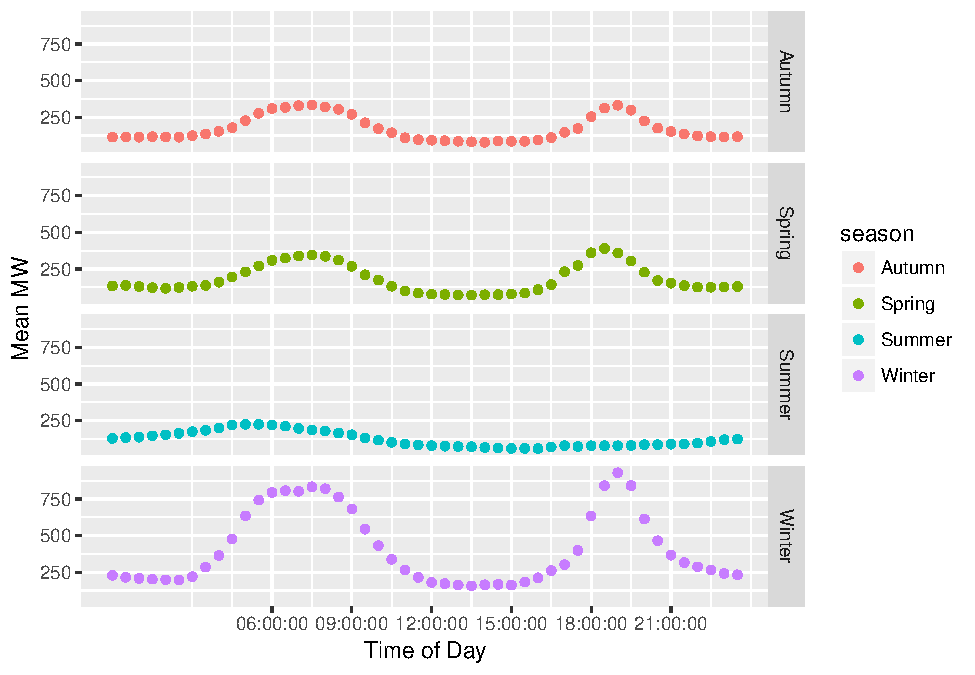
\includegraphics{heatPumpProfileAnalysis_files/figure-latex/aggregateMethod1-1.pdf}

\subsection{Method 2}\label{method-2}

Used the EECA total NZ number for heat pump energy consumption and
converted it into GWh. Converted minute data into half-hour steps. To do
:-)

\begin{quote}
NB: should you aggregate this scaling method using mean or sum? Why? :-)
--\textgreater{}Since we take the percentages of GWh we need to sum up
\end{quote}

\begin{Shaded}
\begin{Highlighting}[]
\CommentTok{# aggregate the percentage of GWh}
\NormalTok{method2AggDT <-}\StringTok{ }\NormalTok{heatPumpProfileDT[, .(}\DataTypeTok{GWh =} \KeywordTok{sum}\NormalTok{(EECApmMethod2)), }
\NormalTok{                                  keyby =}\StringTok{ }\NormalTok{.(season, obsHalfHour)] }\CommentTok{# <- takes the sum for each category of half hour & season}

\NormalTok{myPlot <-}\StringTok{ }\NormalTok{ggplot2}\OperatorTok{::}\KeywordTok{ggplot}\NormalTok{(method2AggDT, }\KeywordTok{aes}\NormalTok{(}\DataTypeTok{x =}\NormalTok{ obsHalfHour, }\DataTypeTok{colour=}\NormalTok{GWh)) }\OperatorTok{+}
\StringTok{  }\KeywordTok{geom_step}\NormalTok{(}\KeywordTok{aes}\NormalTok{(}\DataTypeTok{y =}\NormalTok{ GWh)) }\OperatorTok{+}
\StringTok{  }\KeywordTok{ggtitle}\NormalTok{(}\StringTok{"Total New Zealand half hour heat pump energy consumption by season for 2015"}\NormalTok{) }\OperatorTok{+}
\StringTok{  }\KeywordTok{facet_grid}\NormalTok{(season }\OperatorTok{~}\StringTok{ }\NormalTok{.) }\OperatorTok{+}
\StringTok{  }\KeywordTok{labs}\NormalTok{(}\DataTypeTok{x=}\StringTok{'Time of Day'}\NormalTok{, }\DataTypeTok{y=}\StringTok{'GWh'}\NormalTok{) }\OperatorTok{+}
\StringTok{  }\KeywordTok{scale_x_time}\NormalTok{(}\DataTypeTok{breaks =} \KeywordTok{c}\NormalTok{(hms}\OperatorTok{::}\KeywordTok{as.hms}\NormalTok{(}\StringTok{"00:00:00"}\NormalTok{), hms}\OperatorTok{::}\KeywordTok{as.hms}\NormalTok{(}\StringTok{"03:00:00"}\NormalTok{), hms}\OperatorTok{::}\KeywordTok{as.hms}\NormalTok{(}\StringTok{"06:00:00"}\NormalTok{), hms}\OperatorTok{::}\KeywordTok{as.hms}\NormalTok{(}\StringTok{"09:00:00"}\NormalTok{), hms}\OperatorTok{::}\KeywordTok{as.hms}\NormalTok{(}\StringTok{"12:00:00"}\NormalTok{), }
\NormalTok{                          hms}\OperatorTok{::}\KeywordTok{as.hms}\NormalTok{(}\StringTok{"15:00:00"}\NormalTok{), hms}\OperatorTok{::}\KeywordTok{as.hms}\NormalTok{(}\StringTok{"18:00:00"}\NormalTok{), hms}\OperatorTok{::}\KeywordTok{as.hms}\NormalTok{(}\StringTok{"21:00:00"}\NormalTok{))) }\OperatorTok{+}
\KeywordTok{scale_colour_gradient}\NormalTok{(}\DataTypeTok{low=} \StringTok{"green"}\NormalTok{, }\DataTypeTok{high=}\StringTok{"red"}\NormalTok{)}

\NormalTok{myPlot}
\end{Highlighting}
\end{Shaded}

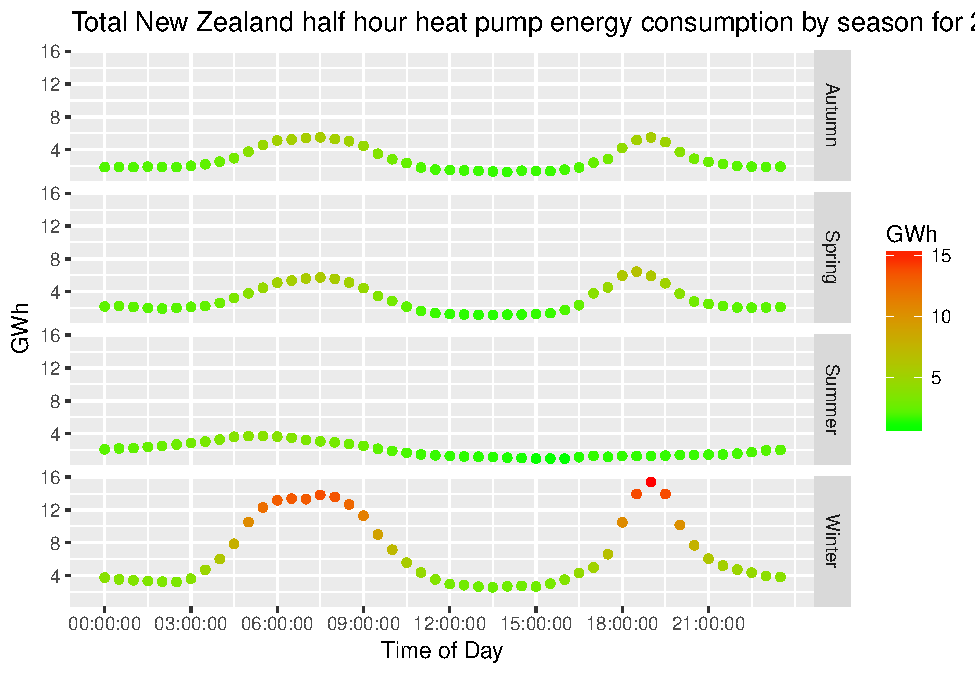
\includegraphics{heatPumpProfileAnalysis_files/figure-latex/aggregateMethod2-1.pdf}

\section{BRANZ vs.~EECA comparison}\label{branz-vs.eeca-comparison}

\begin{Shaded}
\begin{Highlighting}[]
\NormalTok{nzHHheatPumps <-}\StringTok{ }\DecValTok{515015} \CommentTok{#This is based on the BRANZ report of household ownership and 2013 census data}
\NormalTok{wToKw <-}\StringTok{ }\DecValTok{1000}
\NormalTok{assumeDaysPerSeason <-}\StringTok{ }\DecValTok{90}

\NormalTok{heatPumpProfileDT <-}\StringTok{ }\NormalTok{heatPumpProfileDT[, scaledGWh }\OperatorTok{:}\ErrorTok{=}\StringTok{ }\NormalTok{(((meanW }\OperatorTok{*}\StringTok{ }\NormalTok{nzHHheatPumps)}\OperatorTok{/}\NormalTok{wToKw)}\OperatorTok{*}\NormalTok{(}\DecValTok{1}\OperatorTok{/}\DecValTok{60}\NormalTok{)}\OperatorTok{*}\NormalTok{assumeDaysPerSeason)}\OperatorTok{/}\DecValTok{1000}\OperatorTok{/}\DecValTok{1000}\NormalTok{] }\CommentTok{# <- convert mean W to kWh for all NZ hhs, then assumes 90 days per season and calculate GWh}

\NormalTok{sumbranzGWh <-}\StringTok{ }\NormalTok{heatPumpProfileDT[, }\KeywordTok{sum}\NormalTok{(scaledGWh)]}


\NormalTok{diffbranzeeca <-}\StringTok{ }\DecValTok{1}\OperatorTok{-}\NormalTok{(sumbranzGWh}\OperatorTok{/}\NormalTok{totalGWH)}
\NormalTok{skimr}\OperatorTok{::}\KeywordTok{skim}\NormalTok{(sumbranzGWh)}
\end{Highlighting}
\end{Shaded}

\begin{verbatim}
## 
## Skim summary statistics
## 
## -- Variable type:numeric -------------------------------------------------------------------------------------------------------------------
##     variable missing complete n   mean sd     p0    p25    p50    p75
##  sumbranzGWh       0        1 1 638.63 NA 638.63 638.63 638.63 638.63
##    p100     hist
##  638.63 ▁▁▁▇▁▁▁▁
\end{verbatim}

\begin{Shaded}
\begin{Highlighting}[]
\NormalTok{skimr}\OperatorTok{::}\KeywordTok{skim}\NormalTok{(totalGWH)}
\end{Highlighting}
\end{Shaded}

\begin{verbatim}
## 
## Skim summary statistics
## 
## -- Variable type:numeric -------------------------------------------------------------------------------------------------------------------
##  variable missing complete n mean sd  p0 p25 p50 p75 p100     hist
##  totalGWH       0        1 1  708 NA 708 708 708 708  708 ▁▁▁▇▁▁▁▁
\end{verbatim}

\begin{Shaded}
\begin{Highlighting}[]
\NormalTok{skimr}\OperatorTok{::}\KeywordTok{skim}\NormalTok{(diffbranzeeca)}
\end{Highlighting}
\end{Shaded}

\begin{verbatim}
## 
## Skim summary statistics
## 
## -- Variable type:numeric -------------------------------------------------------------------------------------------------------------------
##       variable missing complete n  mean sd    p0   p25   p50   p75  p100
##  diffbranzeeca       0        1 1 0.098 NA 0.098 0.098 0.098 0.098 0.098
##      hist
##  ▁▁▁▇▁▁▁▁
\end{verbatim}

Wee identify that BRANZ in comination with GREENGrid Grid Spy and 2013
household ownership census data represent a 9\% lower total energy
consumption for heat pumps than EECA calculates.

EECA total energy consumption by heat pumps for 2015 (totalGWH)
\textless{}- 708GWh

BRANZ 40\% of owner-occupied households and 25\% of rentals own heat
pumps. Energy consumption based on BRANZ proportion, Census 2013 and
GREENGris Grid Spy data (sumbranzGWh) \textless{}- 638GWh

\section{Yearly consumption}\label{yearly-consumption}

We need the original data for this, currently the data basis is for an
average day in each season.

\begin{Shaded}
\begin{Highlighting}[]
\NormalTok{heatPumpProfileDT <-}\StringTok{ }\NormalTok{heatPumpProfileDT[, obsHalfHour }\OperatorTok{:}\ErrorTok{=}\StringTok{ }\NormalTok{hms}\OperatorTok{::}\KeywordTok{trunc_hms}\NormalTok{(obsHourMin, }\DecValTok{1800}\NormalTok{)]}
\end{Highlighting}
\end{Shaded}

\section{Technical potential of demand response: Scenarios for heat pump
data}\label{technical-potential-of-demand-response-scenarios-for-heat-pump-data}

We assume that peak time periods are prevalent from half hours 13-20 and
32-41, equivalent to 6.30am-10am and 4pm-8.30pm. \#\# Load curtailment
to zero In this first scenario we assume that the laod during peak time
periods is cut out of the consumption pattern.

Steps: 1) Extracting peak time-periods from heat pump data 2) Building
sum of GWh

\begin{Shaded}
\begin{Highlighting}[]
\NormalTok{sc1data <-}\StringTok{ }\NormalTok{heatPumpProfileDT}
\NormalTok{sc1data[, }\KeywordTok{c}\NormalTok{(}\StringTok{"medianW"}\NormalTok{, }\StringTok{"obsHourMin"}\NormalTok{, }\StringTok{"meanW"}\NormalTok{, }\StringTok{"nObs"}\NormalTok{, }\StringTok{"sdW"}\NormalTok{, }\StringTok{"scaledMWmethod1"}\NormalTok{, }\StringTok{"EECApmMethod2"}\NormalTok{)}\OperatorTok{:}\ErrorTok{=}\OtherTok{NULL}\NormalTok{] }\CommentTok{#Deleting unnecessary columns}

\NormalTok{sc1data <-}\StringTok{ }\NormalTok{sc1data[, timePeriod }\OperatorTok{:}\ErrorTok{=}\StringTok{ "Not Peak"}\NormalTok{]}

\NormalTok{sc1data <-}\StringTok{ }\NormalTok{sc1data[obsHalfHour }\OperatorTok{>=}\StringTok{ }\NormalTok{hms}\OperatorTok{::}\KeywordTok{as.hms}\NormalTok{(}\StringTok{"06:30:00"}\NormalTok{) }\OperatorTok{&}\StringTok{ }
\StringTok{                     }\NormalTok{obsHalfHour }\OperatorTok{<=}\StringTok{ }\NormalTok{hms}\OperatorTok{::}\KeywordTok{as.hms}\NormalTok{(}\StringTok{"10:00:00"}\NormalTok{),}
\NormalTok{                   timePeriod }\OperatorTok{:}\ErrorTok{=}\StringTok{ "Morning Peak"}\NormalTok{]}

\NormalTok{sc1data <-}\StringTok{ }\NormalTok{sc1data[obsHalfHour }\OperatorTok{>=}\StringTok{ }\NormalTok{hms}\OperatorTok{::}\KeywordTok{as.hms}\NormalTok{(}\StringTok{"16:00:00"}\NormalTok{) }\OperatorTok{&}\StringTok{ }
\StringTok{                     }\NormalTok{obsHalfHour }\OperatorTok{<=}\StringTok{ }\NormalTok{hms}\OperatorTok{::}\KeywordTok{as.hms}\NormalTok{(}\StringTok{"20:30:00"}\NormalTok{),}
\NormalTok{                   timePeriod }\OperatorTok{:}\ErrorTok{=}\StringTok{ "Evening Peak"}\NormalTok{]}

\NormalTok{sc1data[, .(}\DataTypeTok{sum =} \KeywordTok{sum}\NormalTok{(scaledGWh)), keyby =}\StringTok{ }\NormalTok{.(season, timePeriod)]}
\end{Highlighting}
\end{Shaded}

\begin{verbatim}
##     season   timePeriod       sum
##  1: Autumn Evening Peak  31.74000
##  2: Autumn Morning Peak  33.72567
##  3: Autumn     Not Peak  58.17214
##  4: Spring Evening Peak  38.35552
##  5: Spring Morning Peak  34.48746
##  6: Spring     Not Peak  58.44770
##  7: Summer Evening Peak  11.39316
##  8: Summer Morning Peak  19.99209
##  9: Summer     Not Peak  56.01087
## 10: Winter Evening Peak  82.22371
## 11: Winter Morning Peak  85.00968
## 12: Winter     Not Peak 129.07319
\end{verbatim}

\begin{Shaded}
\begin{Highlighting}[]
\NormalTok{myPlot <-}\StringTok{ }\NormalTok{ggplot2}\OperatorTok{::}\KeywordTok{ggplot}\NormalTok{(sc1data, }\KeywordTok{aes}\NormalTok{(}\DataTypeTok{x =}\NormalTok{ obsHalfHour, }\DataTypeTok{colour=}\NormalTok{scaledGWh)) }\OperatorTok{+}
\StringTok{  }\KeywordTok{geom_step}\NormalTok{(}\KeywordTok{aes}\NormalTok{(}\DataTypeTok{y=}\NormalTok{scaledGWh)) }\OperatorTok{+}
\StringTok{  }\KeywordTok{ggtitle}\NormalTok{(}\StringTok{"Total New Zealand half hour heat pump energy consumption by season for 2015"}\NormalTok{) }\OperatorTok{+}
\StringTok{  }\KeywordTok{facet_grid}\NormalTok{(season }\OperatorTok{~}\StringTok{ }\NormalTok{.) }\OperatorTok{+}
\StringTok{  }\KeywordTok{labs}\NormalTok{(}\DataTypeTok{x=}\StringTok{'Time of Day'}\NormalTok{, }\DataTypeTok{y=}\StringTok{'GWh'}\NormalTok{) }\OperatorTok{+}
\StringTok{  }\KeywordTok{scale_x_time}\NormalTok{(}\DataTypeTok{breaks =} \KeywordTok{c}\NormalTok{(hms}\OperatorTok{::}\KeywordTok{as.hms}\NormalTok{(}\StringTok{"00:00:00"}\NormalTok{), hms}\OperatorTok{::}\KeywordTok{as.hms}\NormalTok{(}\StringTok{"03:00:00"}\NormalTok{), hms}\OperatorTok{::}\KeywordTok{as.hms}\NormalTok{(}\StringTok{"06:00:00"}\NormalTok{), hms}\OperatorTok{::}\KeywordTok{as.hms}\NormalTok{(}\StringTok{"09:00:00"}\NormalTok{), hms}\OperatorTok{::}\KeywordTok{as.hms}\NormalTok{(}\StringTok{"12:00:00"}\NormalTok{), }
\NormalTok{                          hms}\OperatorTok{::}\KeywordTok{as.hms}\NormalTok{(}\StringTok{"15:00:00"}\NormalTok{), hms}\OperatorTok{::}\KeywordTok{as.hms}\NormalTok{(}\StringTok{"18:00:00"}\NormalTok{), hms}\OperatorTok{::}\KeywordTok{as.hms}\NormalTok{(}\StringTok{"21:00:00"}\NormalTok{))) }\OperatorTok{+}
\KeywordTok{scale_colour_gradient}\NormalTok{(}\DataTypeTok{low=} \StringTok{"green"}\NormalTok{, }\DataTypeTok{high=}\StringTok{"red"}\NormalTok{)}

\NormalTok{myPlot}
\end{Highlighting}
\end{Shaded}

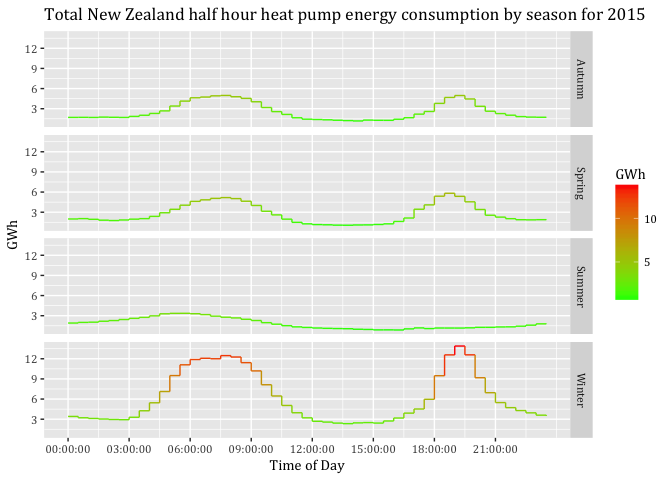
\includegraphics{heatPumpProfileAnalysis_files/figure-latex/scenario load curtailment-1.pdf}

\section{Runtime}\label{runtime}

Analysis completed in 5.83 seconds ( 0.1 minutes) using
\href{https://cran.r-project.org/package=knitr}{knitr} in
\href{http://www.rstudio.com}{RStudio} with R version 3.4.4 (2018-03-15)
running on x86\_64-apple-darwin15.6.0.

\section{R environment}\label{r-environment}

R packages used:

\begin{itemize}
\tightlist
\item
  base R - for the basics (R Core Team 2016)
\item
  data.table - for fast (big) data handling (Dowle et al. 2015)
\item
  lubridate - date manipulation (Grolemund and Wickham 2011)
\item
  ggplot2 - for slick graphics (Wickham 2009)
\item
  readr - for csv reading/writing (Wickham, Hester, and Francois 2016)
\item
  skimr - for skim (Arino de la Rubia et al. 2017)
\item
  knitr - to create this document \& neat tables (Xie 2016)
\item
  nzGREENGrid - for local NZ GREEN Grid project utilities
\end{itemize}

Session info:

\begin{verbatim}
## R version 3.4.4 (2018-03-15)
## Platform: x86_64-apple-darwin15.6.0 (64-bit)
## Running under: macOS High Sierra 10.13.4
## 
## Matrix products: default
## BLAS: /Library/Frameworks/R.framework/Versions/3.4/Resources/lib/libRblas.0.dylib
## LAPACK: /Library/Frameworks/R.framework/Versions/3.4/Resources/lib/libRlapack.dylib
## 
## locale:
## [1] en_NZ.UTF-8/en_NZ.UTF-8/en_NZ.UTF-8/C/en_NZ.UTF-8/en_NZ.UTF-8
## 
## attached base packages:
## [1] stats     graphics  grDevices utils     datasets  methods   base     
## 
## other attached packages:
## [1] bindrcpp_0.2.2      knitr_1.20          skimr_1.0.3        
## [4] hms_0.4.2           readr_1.1.1         lubridate_1.7.4    
## [7] ggplot2_2.2.1       data.table_1.10.4-3 nzGREENGrid_0.1.0  
## 
## loaded via a namespace (and not attached):
##  [1] Rcpp_0.12.16      highr_0.6         pillar_1.2.1     
##  [4] compiler_3.4.4    plyr_1.8.4        bindr_0.1.1      
##  [7] prettyunits_1.0.2 tools_3.4.4       progress_1.2.0   
## [10] digest_0.6.15     gtable_0.2.0      evaluate_0.10.1  
## [13] tibble_1.4.2      pkgconfig_2.0.1   rlang_0.2.0      
## [16] cli_1.0.0         rstudioapi_0.7    yaml_2.1.18      
## [19] xfun_0.2          dplyr_0.7.5       stringr_1.3.0    
## [22] rprojroot_1.3-2   grid_3.4.4        tidyselect_0.2.4 
## [25] glue_1.2.0        R6_2.2.2          rmarkdown_1.9    
## [28] bookdown_0.7      tidyr_0.8.1       purrr_0.2.5      
## [31] reshape2_1.4.3    magrittr_1.5      scales_0.5.0     
## [34] backports_1.1.2   htmltools_0.3.6   assertthat_0.2.0 
## [37] colorspace_1.3-2  labeling_0.3      stringi_1.1.7    
## [40] lazyeval_0.2.1    munsell_0.4.3     crayon_1.3.4
\end{verbatim}

\section*{References}\label{references}
\addcontentsline{toc}{section}{References}

\hypertarget{refs}{}
\hypertarget{ref-skimr}{}
Arino de la Rubia, Eduardo, Hao Zhu, Shannon Ellis, Elin Waring, and
Michael Quinn. 2017. \emph{Skimr: Skimr}.
\url{https://github.com/ropenscilabs/skimr}.

\hypertarget{ref-data.table}{}
Dowle, M, A Srinivasan, T Short, S Lianoglou with contributions from R
Saporta, and E Antonyan. 2015. \emph{Data.table: Extension of
Data.frame}. \url{https://CRAN.R-project.org/package=data.table}.

\hypertarget{ref-lubridate}{}
Grolemund, Garrett, and Hadley Wickham. 2011. ``Dates and Times Made
Easy with lubridate.'' \emph{Journal of Statistical Software} 40 (3):
1--25. \url{http://www.jstatsoft.org/v40/i03/}.

\hypertarget{ref-baseR}{}
R Core Team. 2016. \emph{R: A Language and Environment for Statistical
Computing}. Vienna, Austria: R Foundation for Statistical Computing.
\url{https://www.R-project.org/}.

\hypertarget{ref-ggplot2}{}
Wickham, Hadley. 2009. \emph{Ggplot2: Elegant Graphics for Data
Analysis}. Springer-Verlag New York. \url{http://ggplot2.org}.

\hypertarget{ref-readr}{}
Wickham, Hadley, Jim Hester, and Romain Francois. 2016. \emph{Readr:
Read Tabular Data}. \url{https://CRAN.R-project.org/package=readr}.

\hypertarget{ref-knitr}{}
Xie, Yihui. 2016. \emph{Knitr: A General-Purpose Package for Dynamic
Report Generation in R}. \url{https://CRAN.R-project.org/package=knitr}.


\end{document}
